\section{\glsentryshort{pws} Dynamical Systems}
\label{sec:state.discont}

\hl{(Heading changed)}

Initially, the theory of non-linear \hl{dynamical systems} was developed for smooth \hl{dynamical systems} only.
Hence, \hl{several} results can't be applied to \hl{\gls{pws} dynamical} systems.
But smooth systems are not fit to model \hl{several} engineering applications, since \hl{such} systems often undergo sudden changes.
For example, a model for an electrical circuit can't be smooth as soon as the circuit has a single switching element, such as a transistor~\cite{ZhuMos03}.
The model we will investigate in this thesis describes such an electrical circuit.

In \hl{\gls{pws} dynamical systems}, bifurcations are possible, that were not possible in smooth \hl{dynamical} systems.
\hl{Even more so in \gls{pws} discontinuous dynamical systems, which this thesis focuses on.}
While the theory for \hl{continuous-time} 1D \hl{\gls{pws}} discontinuous \hl{dynamical} systems is quite complete, the theory for \hl{time-discrete} 1D \hl{\gls{pws}} discontinuous \hl{dynamical} systems in is further behind~\cite{Simpson16}.
Also while in \hl{smooth dynamical systems and \gls{pws} continuous dynamical systems} bifurcations can be generalized and described using normal forms, this is not possible for \hl{\gls{pws} discontinuous dynamical systems}.
The reason for this is, that many bifurcations, especially \glspl{bcb}, are necessarily global and normal forms only work for local bifurcations.
\todo{citation}
Hence, we will \hl{not construct a normal form in this thesis}.
\hl{
	Rather we will construct a simpler model that shows the same bifurcation structures as the considered complex model.
	We will call this an archetypal model.
}

The bifurcations covered in this thesis all belong to the previously mentioned class of \glspl{bcb}.

\begin{definition}[Border Collision]
	\hl{
		A \glsentrylong{bc} is a point in the parameter space, where an invariant set (e.g. a fixed point or a cycle) collides with a border of the model function in the state space.
		Borders of the model function being discontinuities of the model function.
	}
\end{definition}

\begin{definition}[Border Collision Bifurcation]
	\hl{
		A \glsentrylong{bcb} is a \gls{bc} that also causes a qualitative change in the state space topology.
	}
\end{definition}

\hl{
	Since model functions of \gls{pws} dynamical systems consist of multiple branches, we can describe cycles in such systems using symbolic sequences.
	This allows us to differentiate between different cycles even if they have the same period.
}

\begin{definition}[Symbolic Sequence]
	\hl{
	Let $f: \mathbb{R} \to \mathbb{R}$ be \hl{the model function of a \gls{pws} dynamical system} that is divided into $n$ partitions $I_j$ where $0 \leq j < n$.
	And let the set of symbols associated with each partition $I_j$ be $\left\{S_j\right\}_{0 \leq j < n}$.
	The symbolic sequence $S_f(\O_k)$ of a cycle $\O_k = \left\{x_i \mid 0 \leq i < k\right\}$ is defined in the following way.
	}
	\begin{align}
		S_f(\O_k) = \left(a(x_0), a(x_1), \dots, a(x_{k-1})\right)
	\end{align}
	\hl{
		Where the function $a$ provides a symbol for every point of the cycle.
		It is defined as $a(x) = S_j$ if $x \in S_j$ for all $0 \leq j < n$~\cite{granados14adding}.
	}
\end{definition}

\hl{
	We will now introduce a class of bifurcation structures that this thesis covers towards the end in \Cref{chap:add}.
	Bifurcation structures belonging to this class can be found in many \gls{pws} dynamical systems, and they are called period-adding structures.
}

Period-adding structures are named like this because in such structures, between a parameter region with a cycle of period $a$ and another parameter region with a cycle of period $b$, there is a parameter region with a cycle of period $a + b$.

\todo{Replace pic with $\L$ and $\R$ adding}
\begin{figure}
	\centering
	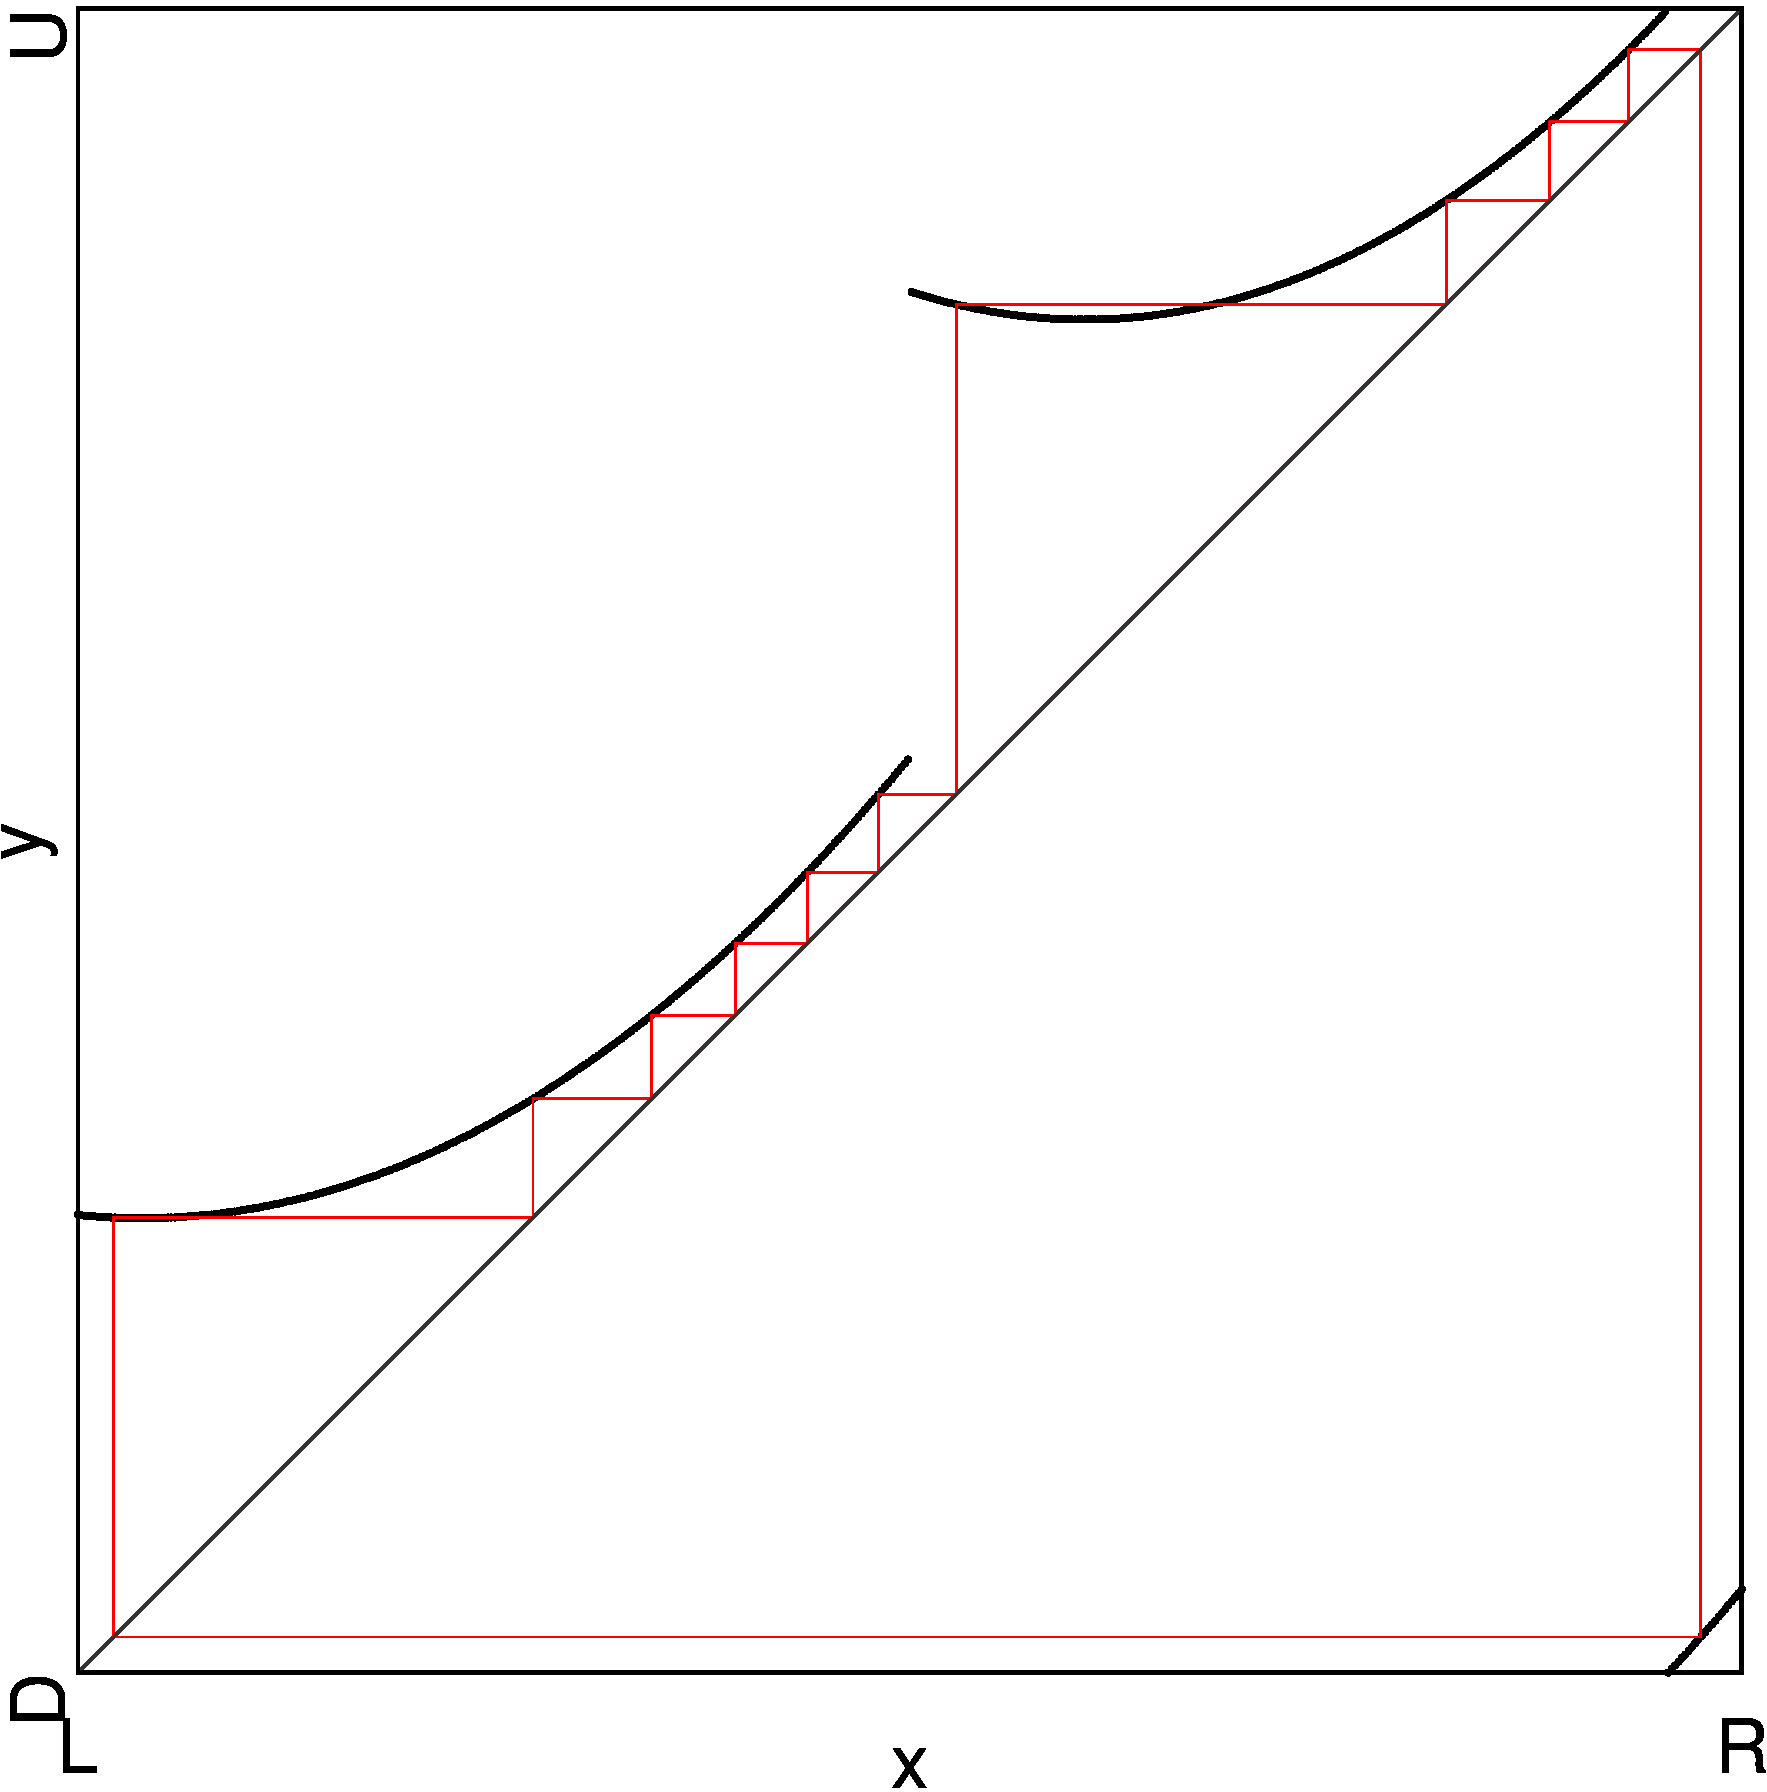
\includegraphics[width=.5 \textwidth]{80_Adding_LR/1D_Period/result.png}
	\caption[1D scan of periods in a period-adding structure between $\L$ and $\R$]{
		1D scan of the periods of cycles in a period-adding structure with the starting cycles $\L$ and $\R$.
	}
\end{figure}

\hl{
	An even more compact way to differentiate between multiple cycles that have the same period are rotation number.
	Here, we will use them to describe the structure of period-adding structures.
}

\begin{definition}[Rotation Numbers --- Keener]
	Let $\sigma$ be a cycle of a \gls{pws} dynamical system $x_{n+1} = f(x_n)$ with two branches, $\L$ and $\R$.
	Then the rotation number $\rho(\sigma)$ of this cycle is defined as the ratio of the symbols $\L$ in the symbolic sequence of the cycle $|\sigma|_\L$ divided by the period of the cycle $|\sigma|$~\cite{Keener80}.
	\begin{align}
		\rho(\sigma) = \dfrac{|\sigma|_\L}{|\sigma|}
	\end{align}
\end{definition}

The rotation numbers of the cycles in a period-adding structure are organized in a Farey-tree.
A Farey-tree has two ``root nodes'' and the child node of two nodes is the Farey-sum of the parent nodes~\cite{granados14adding}.

\begin{definition}[Farey-sum]
	The Farey-sum $a \oplus b$ of two fractions $a = \frac{a_1}{a_2}$ and $b = \frac{b_1}{b_2}$ is defined in the following way.
	\begin{align}
		a \oplus b = \frac{a_1}{a_2} \oplus \frac{b_1}{b_2} = \dfrac{a_1 + b_1}{a_2 + b_2}
	\end{align}
\end{definition}

\Cref{fig:state.discont.adding.farey.rot} shows such a Farey-tree of a period-adding structure between two fixed points, $\L$ and $\R$.
If we replace the content of the nodes with the symbolic sequences of the cycles, we get the tree shown in \Cref{fig:state.discont.adding.farey.rot}.
Instead of Farey-addition, here the child node of two parent nodes is the concatenation of the symbolic sequences in the parent nodes.
\hl{Together with \Cref{theorem:state.rot.num.concat}, this explains why} the  tree in \Cref{fig:state.discont.adding.farey.rot} is a Farey-tree~\cite{granados14adding}.

\begin{theorem}[Rotation Numbers of Concatenated Cycles]
	The rotation number of the concatenation of two cycles $\rho(\sigma\varrho)$ is the Farey-sum of the rotation numbers of both cycles, $\rho(\sigma) \oplus \rho(\varrho)$.
	\label{theorem:state.rot.num.concat}
\end{theorem}

\begin{proof}
	\begin{align*}
		\rho(\sigma\varrho)
		= \dfrac{|\sigma\varrho|_\L}{|\sigma\varrho|}
		= \dfrac{|\sigma|_\L + |\varrho|_\L}{|\sigma| + |\varrho|}
		= \dfrac{|\sigma|_\L}{|\sigma|} \oplus \dfrac{|\varrho|_\L}{|\varrho|}
		= \rho(\sigma) \oplus \rho(\varrho)
	\end{align*}
	\vspace{-4.8em}
	\begin{flushright}
		$\blacksquare$
	\end{flushright}
\end{proof}

\begin{figure}
	\centering
	\subfloat[Rotation Numbers]{
		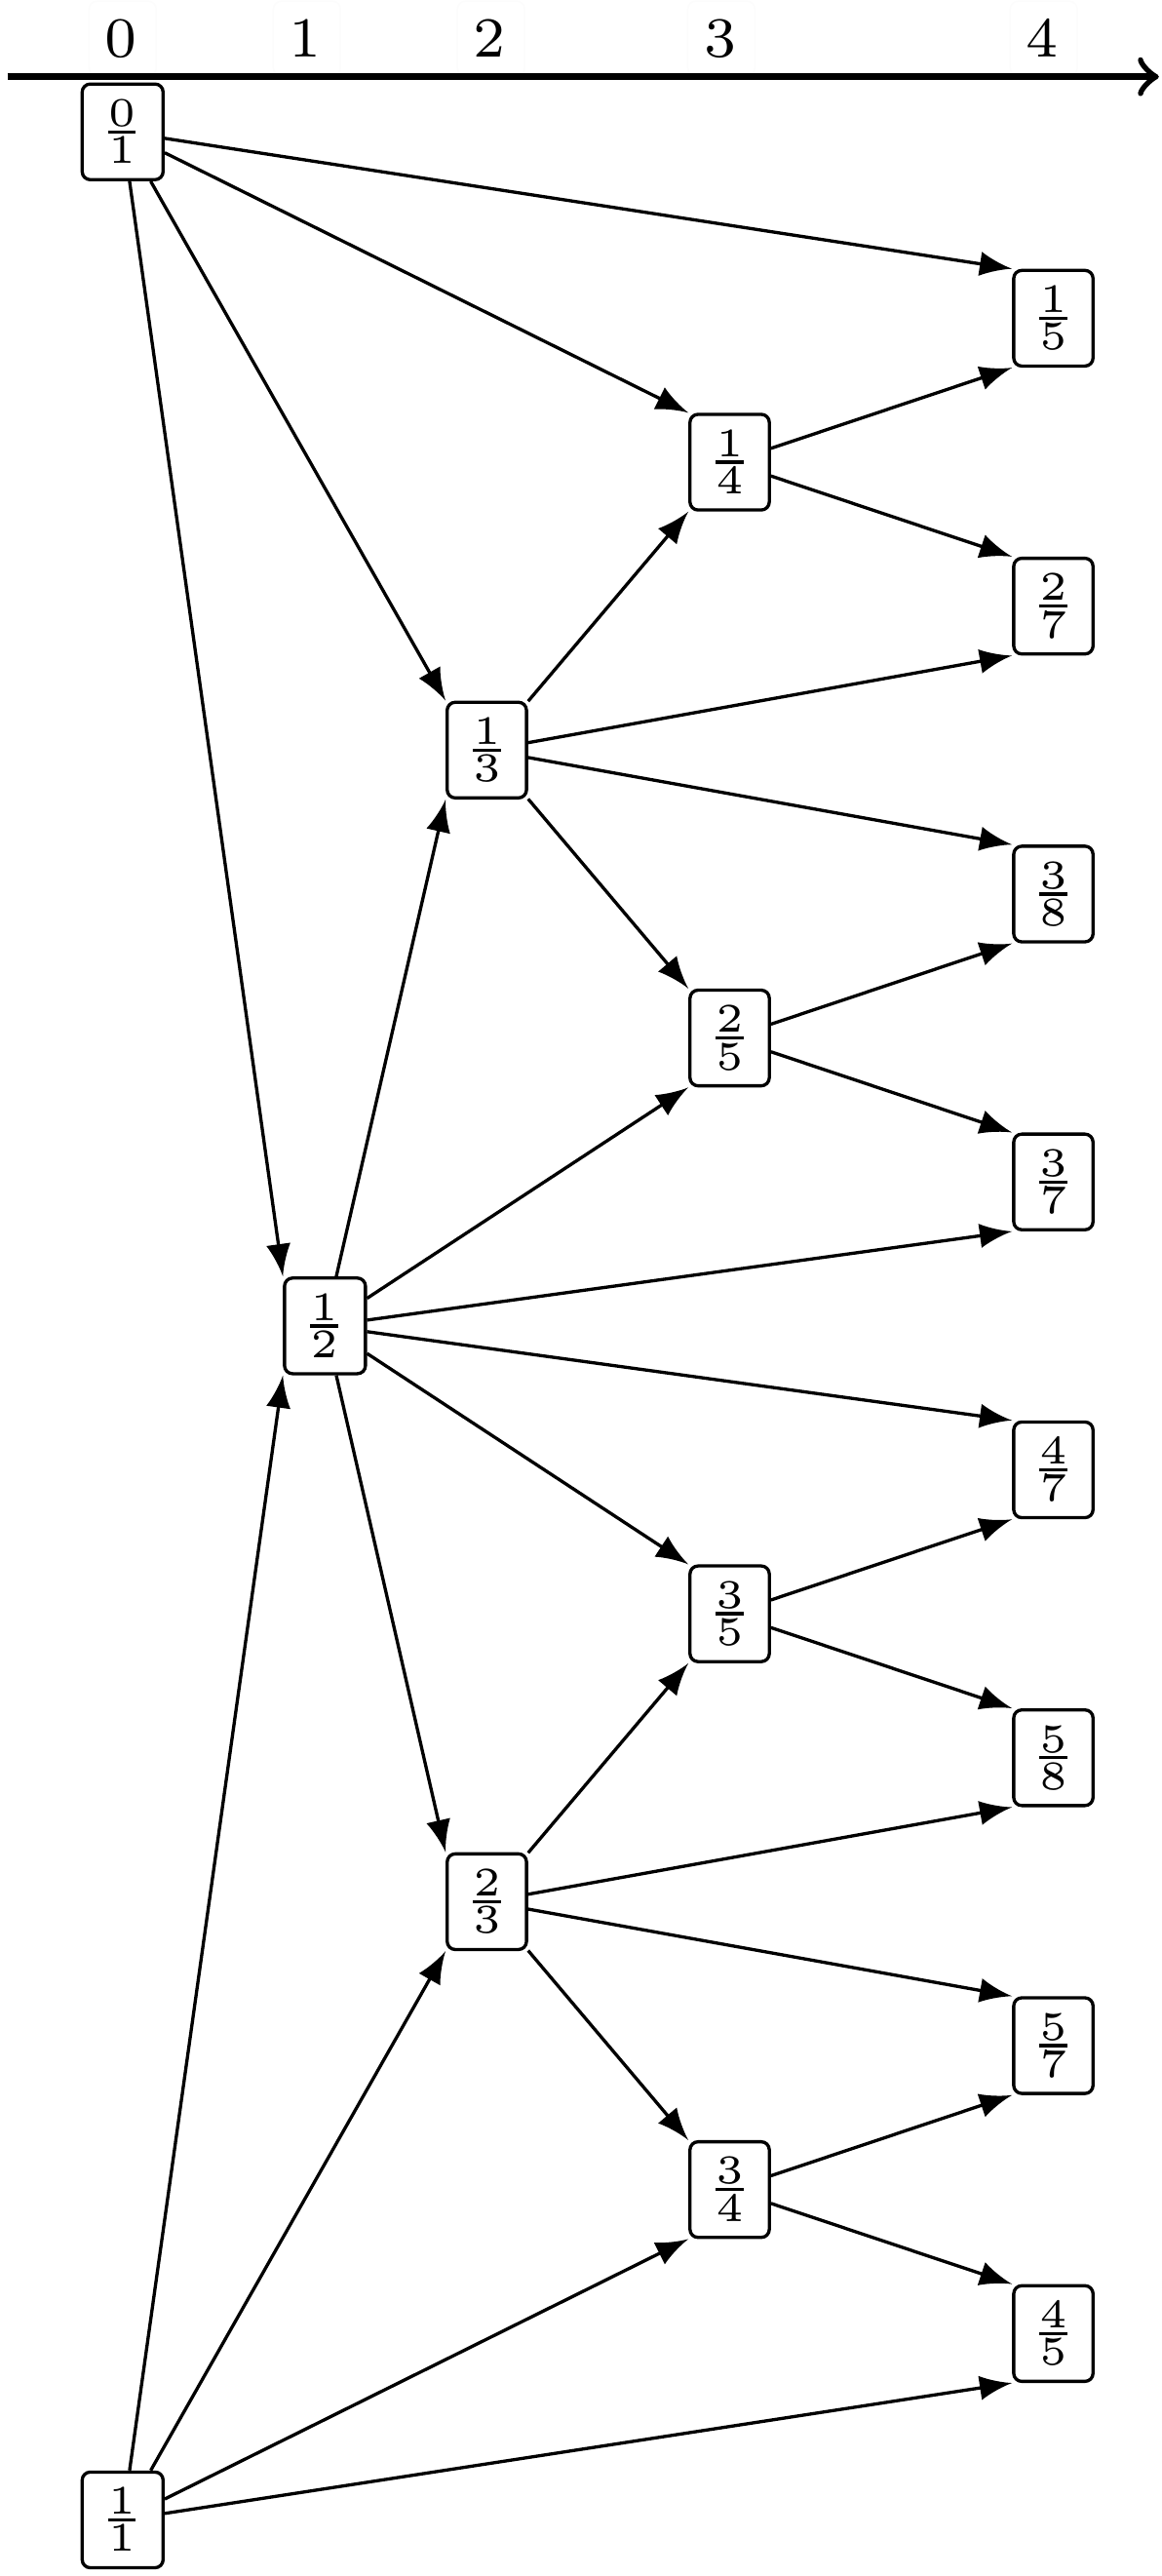
\includegraphics[height=.4 \textheight]{Figures/FareyTrees/LR_RotNum/adding.png}
		\label{fig:state.discont.adding.farey.rot}
	}
	\quad
	\subfloat[Symbolic Sequences]{
		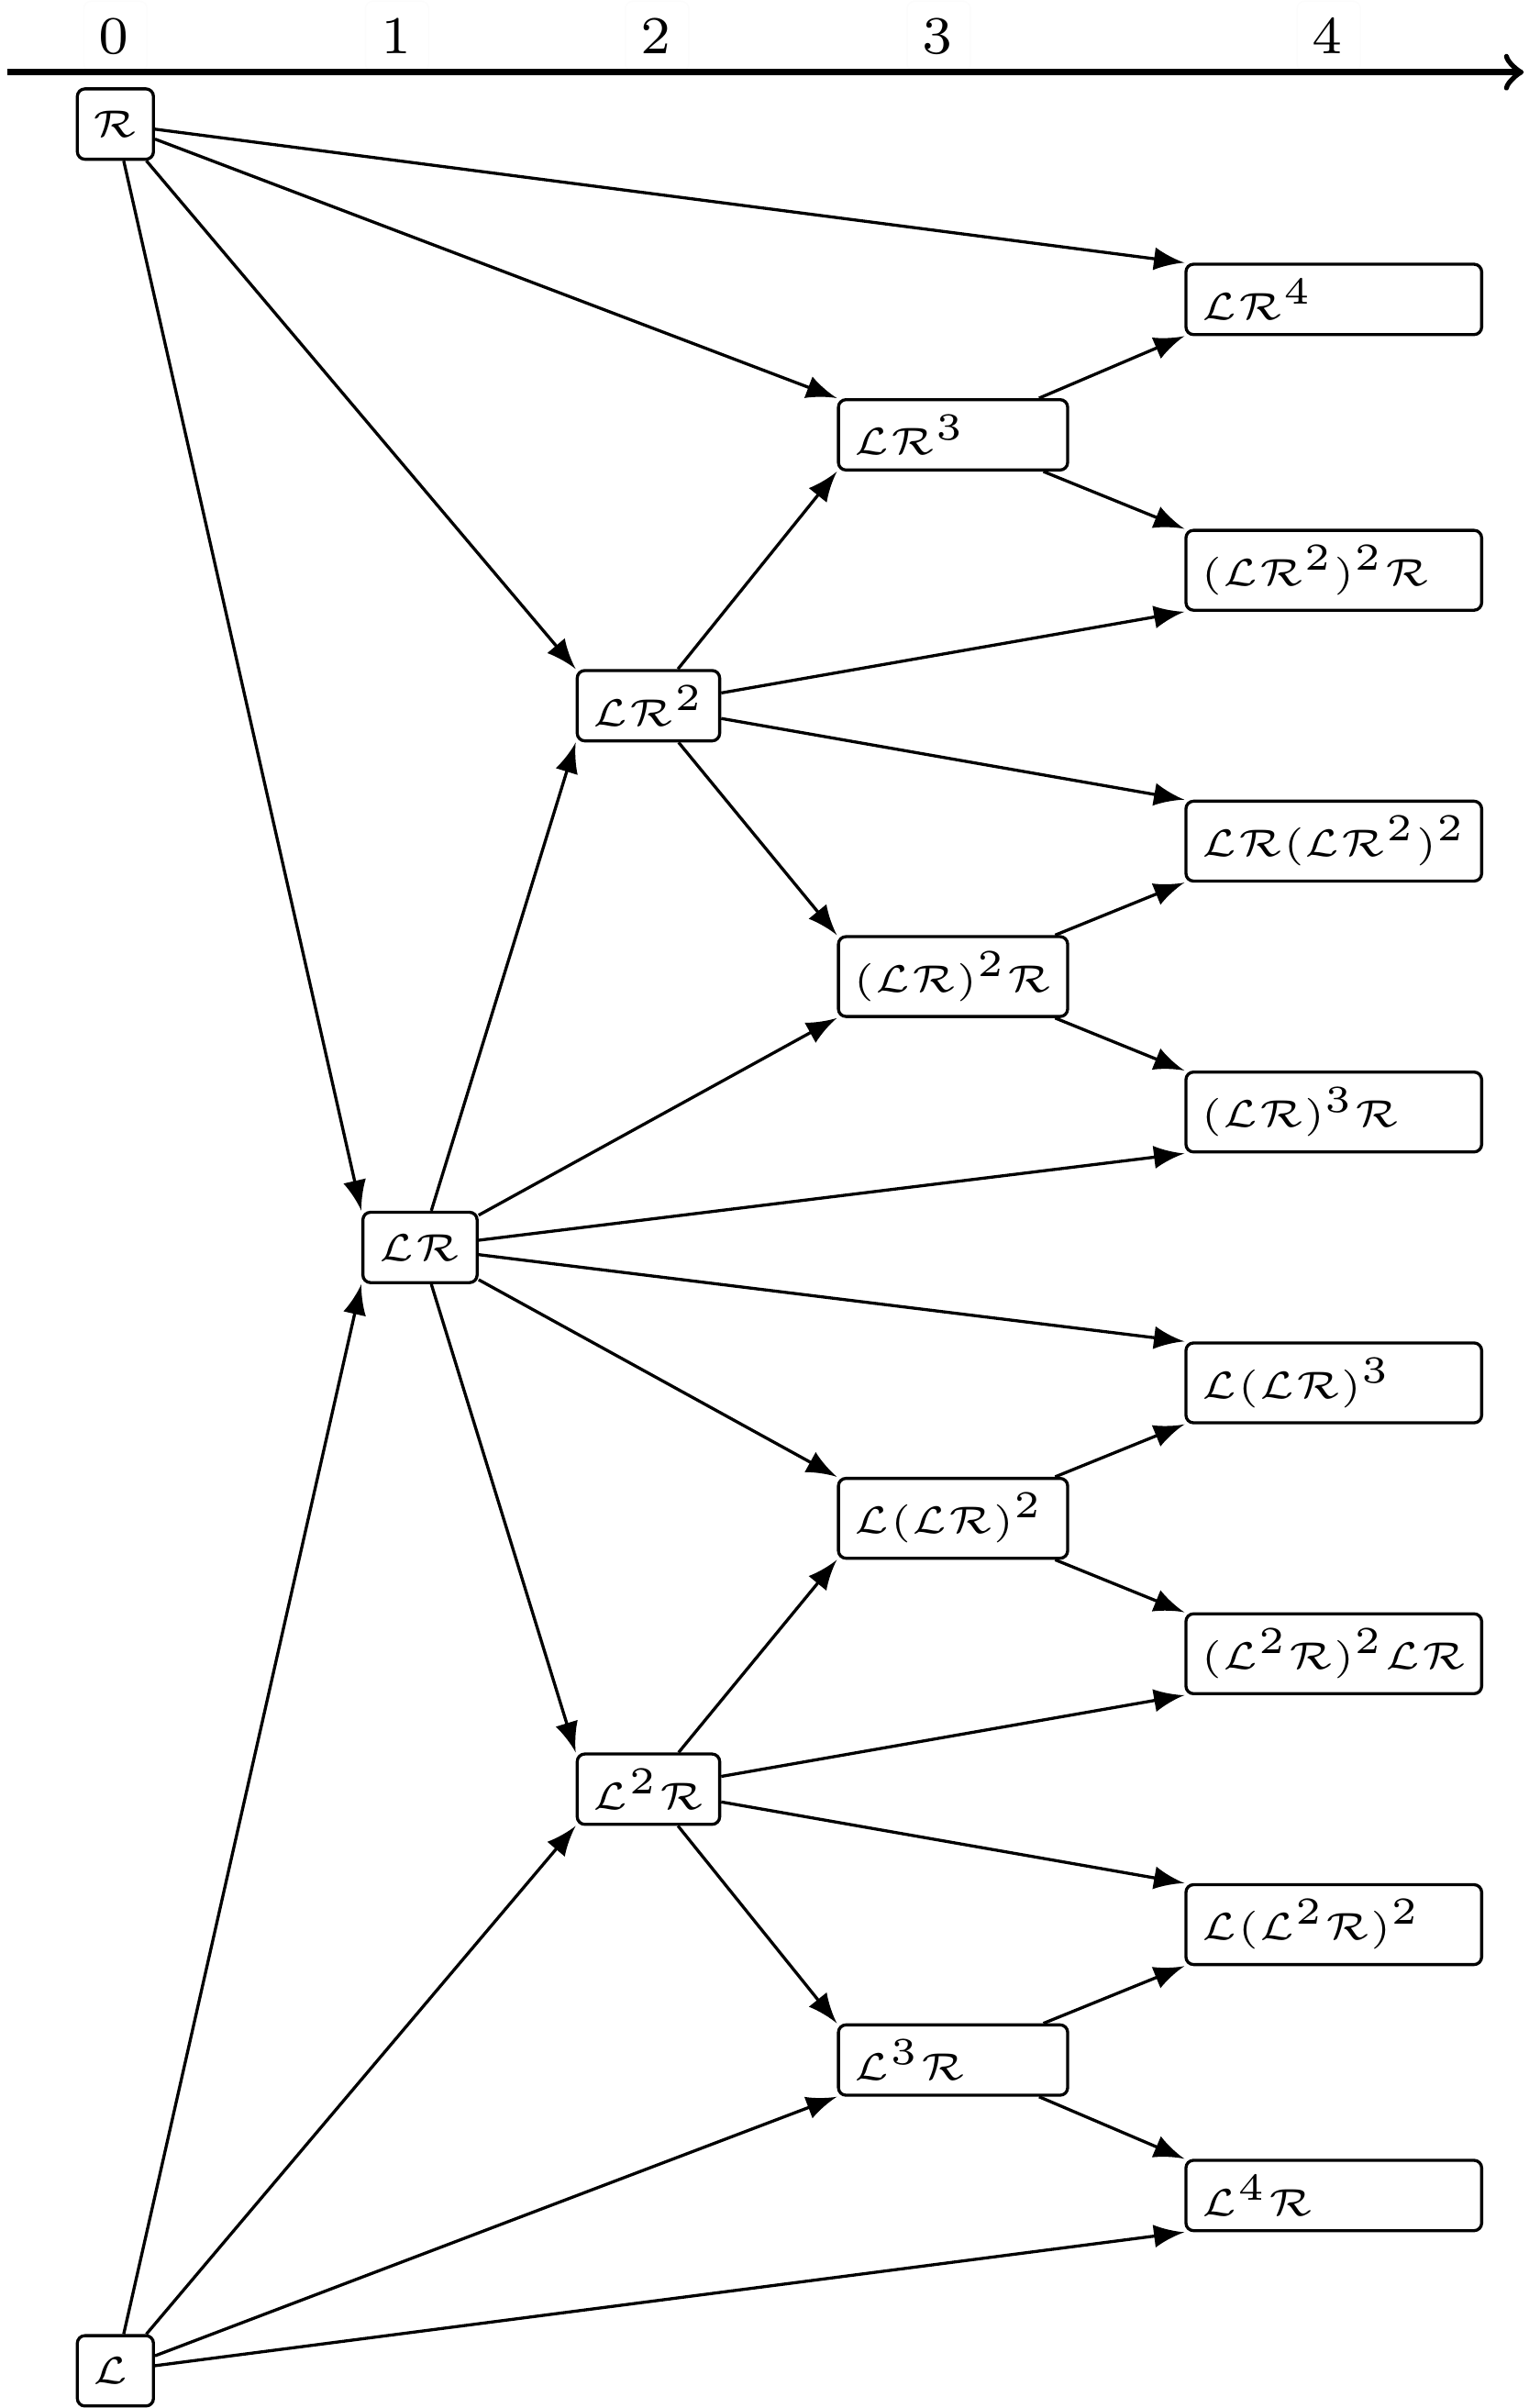
\includegraphics[height=.4 \textheight]{Figures/FareyTrees/LR/adding.png}
		\label{fig:state.discont.adding.farey.sym}
	}
	\caption[Farey-trees of a period-adding structure between $\L$ and $\R$]{
		Farey-trees of a period-adding structure with the starting cycles $\L$ and $\R$.
		(a) Shows the rotation numbers while (b) shows the symbolic sequences of the cycles in this structure.
	}
	\label{fig:state.discont.adding.farey}
\end{figure}
